% -*- TeX:UK -*-
\chapter{Regression of curves: The simplex algorithm}\label{chap:Simplex}
\begin{refsection}

\abstract{The simplex algorithm is an iterative technique that can be used for any regression problem, from straight lines to curves of arbitrary complexity. The differential of the equation need not be known nor even exist. It is not limited to minimising the sum of squared residuals, but can use any optimisation criterium that is continuous. Minimum median residual is used for noisy data, minimum \(\chi^2 \) for heteroscedastic data. The biggest disadvantage of the simplex algorithm is that it does not directly produce error estimates for the parameters, these need to be obtained by bootstrapping. }

\section{How does the simplex algorithm work?}

\begin{figure}
 \caption{RSS of the data in fig. \ref{fig:LinReg} on page \pageref{fig:LinReg} as function of the values of the parameters. Each pair of parameters gives a RSS-value (colour-coded like a topographic map). The black triangles indicate the moves of the simplex from an arbitrary starting point, note how the simplex expands as it moves downhill and then contracts again near the minimum. For details see text. }
 \label{fig:ErrorSurface}
 \centering
 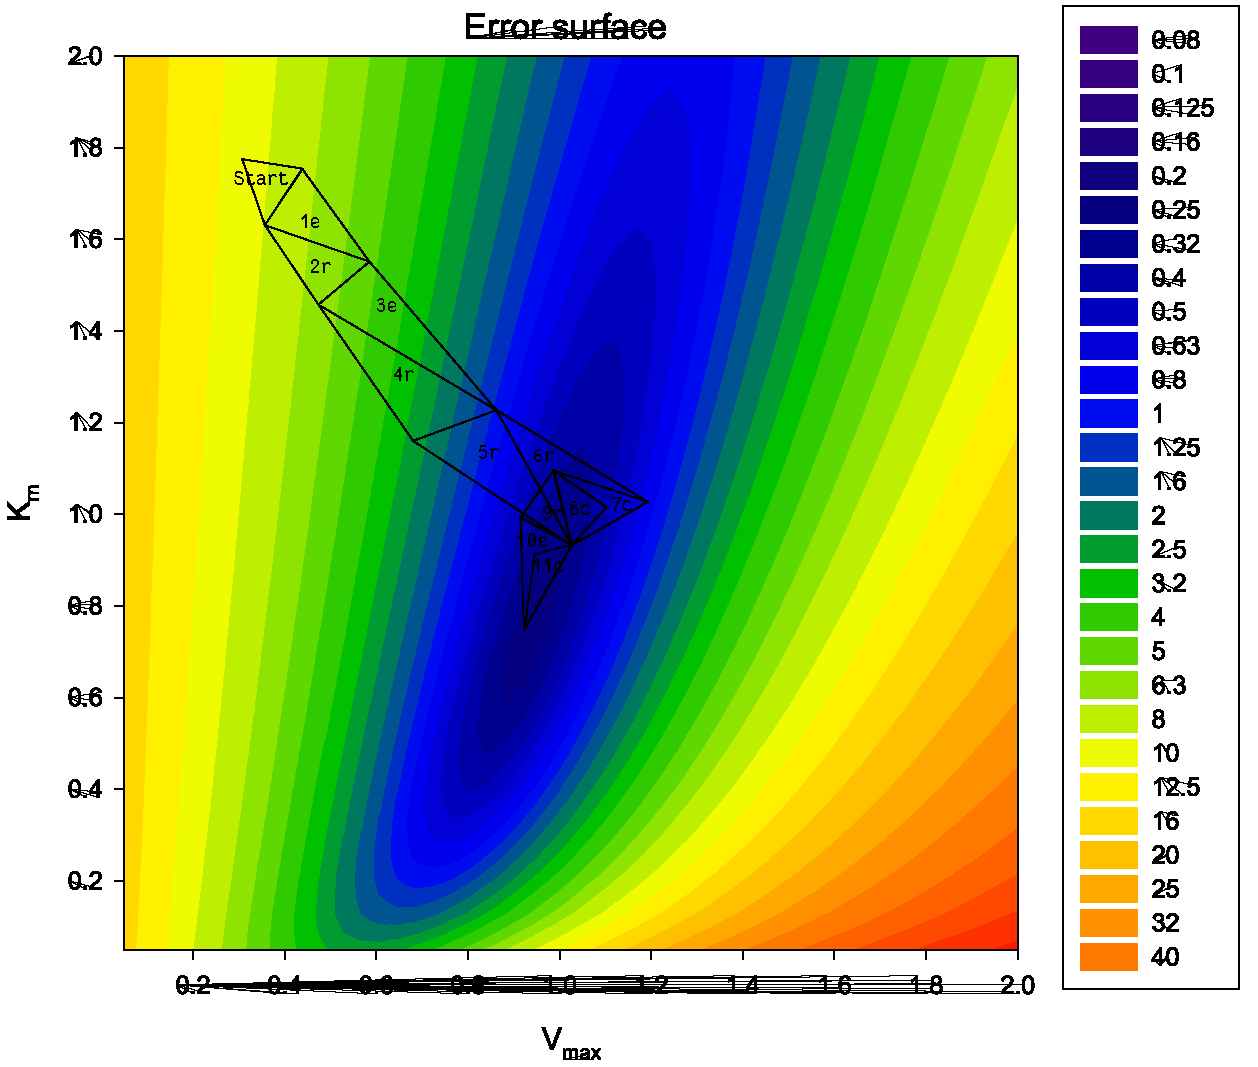
\includegraphics[width=\textwidth]{Graphics/ErrorSurface}
\end{figure}

Let us return to the example in fig. \ref{fig:LinReg} on page \pageref{fig:LinReg}, a \Name{Henri-Michaelis-Menten} curve with considerable scatter. We can now choose arbitrary pairs of the parameters, \skalar{V_\mathrm{max}} and \skalar{K_\mathrm{m}}, each such pair will give a \acf{RSS} (see fig. \ref{fig:ErrorSurface}). What we would like to find is the pair of parameters for which \acs{RSS} becomes minimal. All \acs{RSS}-values of all parameter sets (although we deal with two parameters here for ease of drawing, the method can handle an arbitrary number of parameters \skalar{p}, the error surface then has \(p+1 \) dimensions) together form the \textbf{error surface} of the problem. In effect, we look for way to take an arbitrary starting set of parameters and from there move ``downhill'' until we reached the minimum with sufficient precision. One way of doing this is to calculate the gradient (\skalar{\nabla},  multi-dimensional slope) of the function at your current estimate for the parameters and move downward in the direction to the \textbf{steepest descent} for a small distance, arriving at your new, improved estimate. This is repeated until further moves no longer reduce the \acs{RSS}, that is, until the gradient becomes close to zero. The \Name{Levenberg-Marquardt} \parencite{Lev-44,Mar-63} algorithm uses (in part) this method. However, this requires the error function not only to be continuously differentiable (without singularities as for example in \(f(x) = 1/x, x = 0 \)), but the first derivative must also be known (how good were you in calculus?). The main advantage of steepest descent methods is that since the gradient is known, it is easy to calculate error estimates for the found parameters directly.

The simplex algorithm \parencite{Nel-65,Cac-84,Kim-97} takes a geometric approach, and is therefore more generally applicable. Neither the regression function nor its error surface need to be differentiable, all that is required is that we can calculate the dependent variable \(\hat{\AbsVec{y}} \) for any data vector \(\AbsVec{x} \) and any parameter vector \(\beta \). The simplex method can minimise not only the \acs{RSS}, but also other error functions like \(\chi^2 \) or the median of residuals. This can be useful for non-homoscedastic or noisy data. However, simplex does not directly give error estimates for the parameters, these need be calculated from bootstrapping \parencite{Str-92,Str-10}.

\begin{figure}
 \caption{Possible movements of a simplex. The old simplex is in \emph{green}, the new in \emph{orange}. For details see text. }
 \label{fig:SimMo}
 \centering
 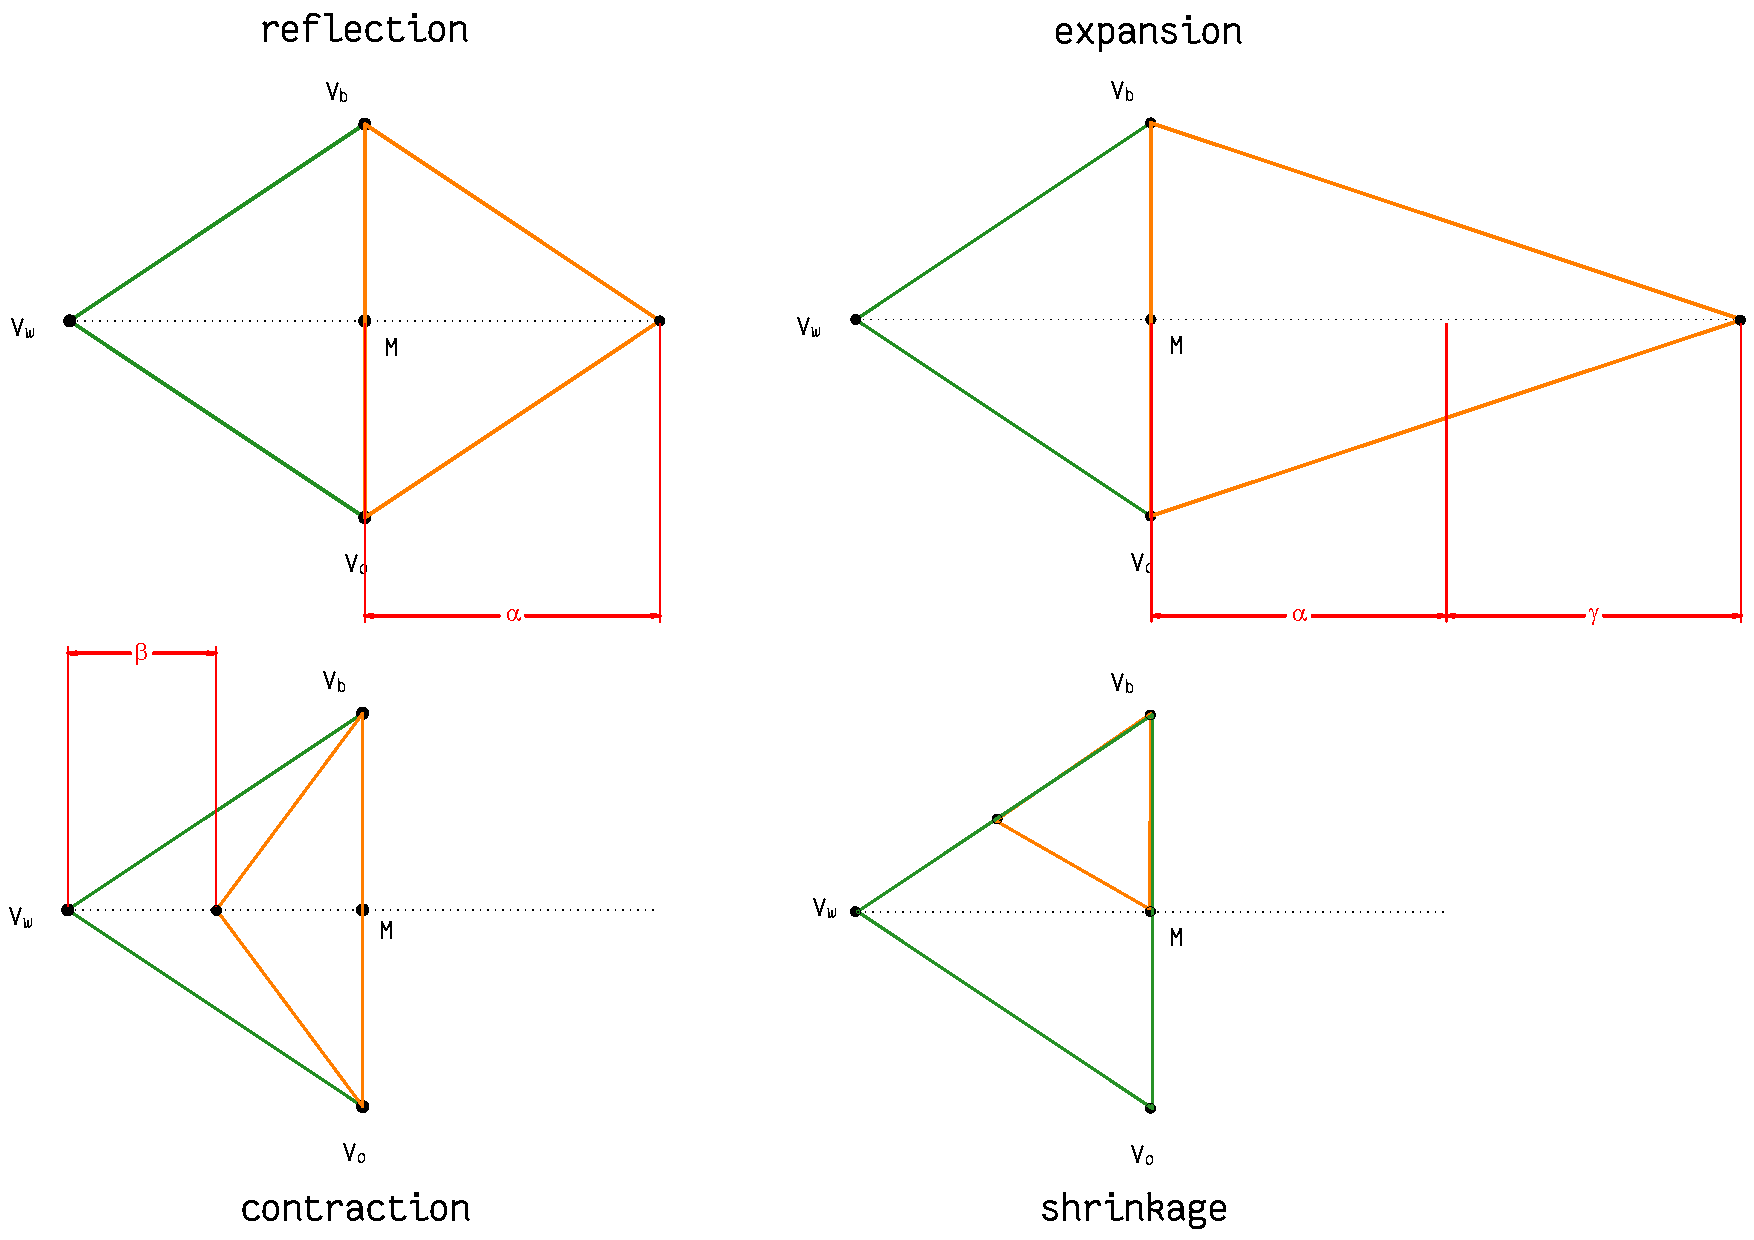
\includegraphics[width=\textwidth]{Graphics/Simplex-moves}
\end{figure}

A simplex is a geometric figure that has one more vertex than the space in which it lives has dimensions. The \skalar{p} Parameters of a fitting problem define a \skalar{p}-dimensional space, in our example we have two parameters, the space hence is a plane and the simplex is a triangle. With tree parameters, the simplex would be a tetrahedron, \Foreign{etc}. Each vertex is characterised by its parameters and, in addition, by the \acs{RSS} associated with it. We then discard the vertex with the highest \acs{RSS}, replacing it with another one with (hopefully) lower \acs{RSS}, so that the vertex ``moves'' downhill. At each step, a vertex can do one of four things (see also fig. \ref{fig:SimMo}):
\begin{description}
  \item[reflection]{move the worst vertex \(V_w \) along the line that connects it to the midpoint \(M \) of the other vertexes for the distance \(\overline{V_wM} + \alpha \overline{V_wM} \). In other words, with \(\alpha = 1 \) the worst vertex is mirrored on the connection between all other vertexes. The new vertex is accepted, if its \acs{RSS} is neither higher than that of \(V_w \), nor lower than that of the best vertex \(V_b \). }
  \item[contraction]{If the \acs{RSS} of the reflected vertex is worse than \(V_w \), the program tries to move this vertex for only \(\beta \overline{V_wM} \). The new vertex is accepted if its \acs{RSS} is lower than that of \(V_w \).}
  \item[expansion]{If the new vertex is better than the previously best vertex \(V_b \), the program tries to move it even further along the line used for reflection, that is for a total of \(\overline{V_wM} + (\alpha+\gamma)\overline{V_wM} \). This expanded vertex is accepted if its \acs{RSS} is lower than that of the discarded \(V_w \).}
  \item[shrinkage]{If in contraction the \acs{RSS} of the new vertex is lower than that of \(V_w \), the program keeps the best vertex and moves all others toward it by half their distance. }
\end{description}
It was shown in \parencite{Kim-97}, however, that shrinkage can never occur, and hence is redundant. The simplex algorithm is guaranteed never to diverge, it is quite efficient as no matrix operations are required. Round-off errors are minimised, but all calculations should be done at least in double precision, with the old Turbo Pascal \texttt{real}-type the algorithm sometimes did not converge, the simplex continued to rotate around the optimum until the maximal number of iterations was reached. To avoid the simplex to become trapped in a local minimum, the starting estimates should be as close to the final parameters as possible. Alternatively, use several -- wildly different -- starting values and verify that they result in the same final parameters.

Instead of \acs{RSS}, other parameters may also be used to control the fit. For noisy data, the median of residuals is more stable against outlying data points. For data with constant relative (rather than absolute) error, \(\chi^2 \) (the sum of squared relative errors) is the appropriate fitting criterium.

\section{Examples}

\subsection{Enzyme kinetics with [S] spanning several orders of magnitude: heteroscedasticity}

\begin{figure}
 \caption{ATPase-activity of Mdr1 as function of [ATP]. The data can be well described by a model with four catalytic and one inhibitory binding site, this results in a ratio of polynoms of 4/5 grade. However, while points at high [ATP] can be fitted by minimising \(\chi^2 \) or RSS, at low concentrations the data can be fitted only with \(\chi^2 \). The data have equal relative error, at low [ATP] the velocities, and hence absolute errors, are so small that they make negligible contribution to \acs{RSS}.}
 \label{fig:ATPase}
 \centering
 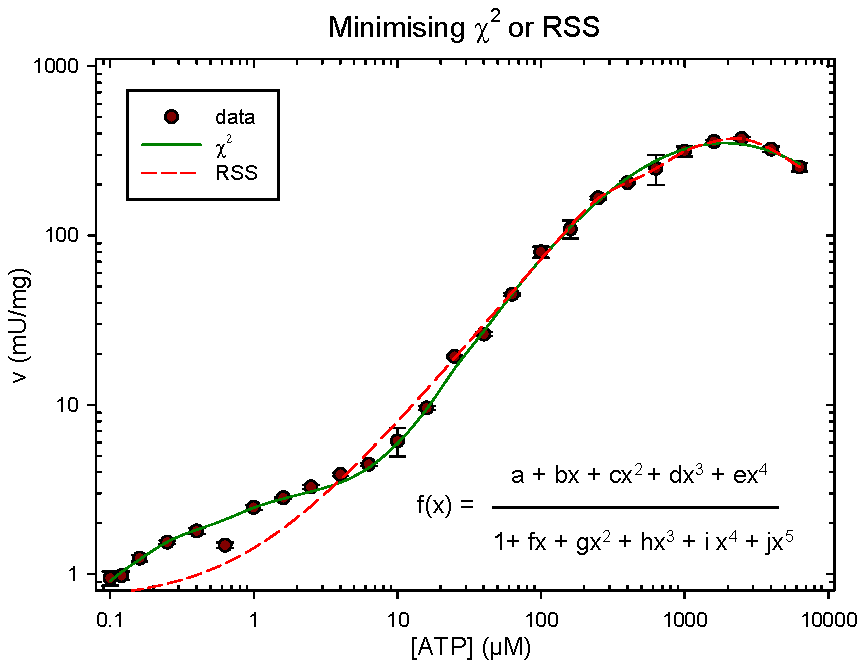
\includegraphics[width=0.75\textwidth]{Graphics/ATPase-chisqr-rss}
\end{figure}

Normally, enzyme kinetics data cover substrate concentrations of two orders of magnitude, between \(0.1 K_m \) and \(10 K_m \). A  minimum of \num{12} data points, equally spaced, in this interval are required for fitting of the \Name{Henri-Michaelis-Menten} (HMM) curve \parencite{Rit-96}. However, some ATPases have several ATP-binding sites with very different \(K_m \). For example, in P-type ATPases like \chemical{Na/K}-ATPase these are \SI{0.1}{\micro M} and \SI{300}{\micro M}, respectively. The question arose, whether ABC-type ATPases like Mdr1, who have two ATP-binding sites in each molecule, would operate with HMM-kinetics, or show cooperativity like the P-type ATPases (where several enzyme molecules with one binding site each have to work together). Therefore, the \( v / [S] \) curve of Mdr1 was measured in the concentration range from \SI{100}{nM} to \SI{10}{mM}, that is, over 5 orders of magnitude \parencite{Bux-99b}. All experiments contained the same amount (\SI{3500}{Bq}) of \textgamma\isotope[33]{P}-ATP as label, but different concentrations of unlabelled ATP, resulting in different specific radioactivity. The formation of \chemical{H}\isotope[33]{P}\chemical{O_4^{2-}} was measured, resulting in velocities that had the same \emph{relative} error. Use of the minimal \acs{RSS} criterion, however, requires data with the same \emph{absolute} error (homoscedasticity). Only minimising \(\chi^2 = \sum_{i=1}^n{\left[\frac{(\hat{\AbsVec{y}}_i - \AbsVec{y}_i)}{\AbsVec{y}_i}\right]^2} \), the sum of squared \emph{relative} errors, allows these data to be fitted, \acs{RSS} fails at low substrate concentrations (see fig. \ref{fig:ATPase}).

\subsection{Fitting of a system of differential equations to a data set}

\begin{figure}
 \caption{System of linear differential equations for the equation A \(\rightarrow \) B \(\rightarrow \) C, the measured values are the intermediate product multiplied by an extraction efficiency (mean and standard deviation of 4 repetitions). For details see text. }
 \label{fig:extract}
 \centering
 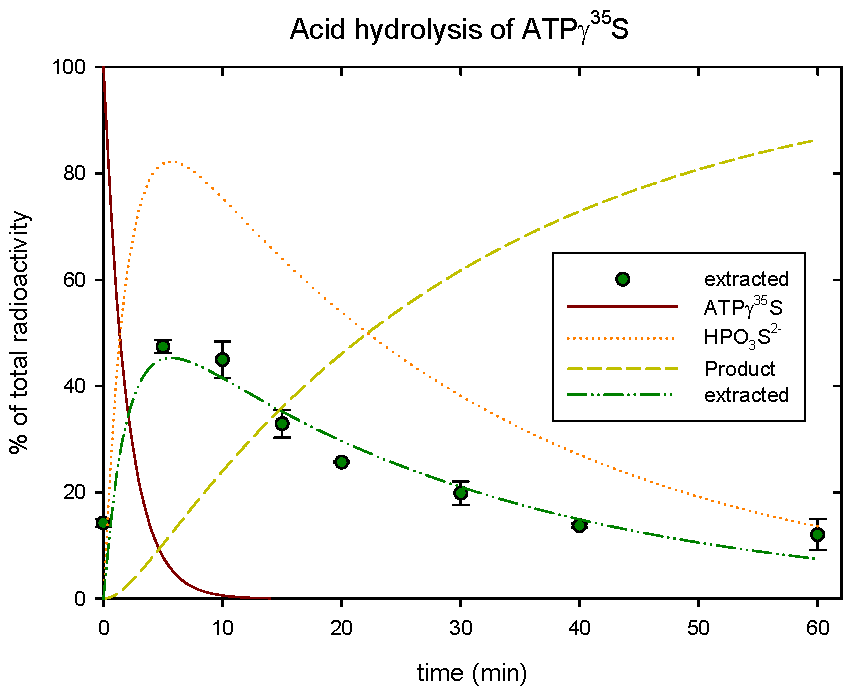
\includegraphics[width=0.75\textwidth]{Graphics/FitSystem}
\end{figure}

The question was whether \SI{70}{kDa} heat shock protein could hydrolyse the ATP-analog ATP\textgamma\isotope[35]{S}. The common method for the determination of \isotope[33]{P}\chemical{O_4^{2-}} is to convert the phosphate to \chemical{(NH_4)_3[P(Mo_3O_{10})_4]} in the presence of carrier phosphate and to extract into organic solvent, the radioactivity in that extract is then counted. To determine whether this method could also be used for thiophosphate, a small amount of ATP\textgamma\isotope[35]{S} was hydrolysed in \SI{2}{N} \chemical{H_2SO_4} at \SI{95}{\celsius}, and samples taken at several time points. Under these conditions, ATP and similar high-energy compounds are hydrolysed quantitatively within \SI{7}{min}. However, it turned out that the thiophosphate is destroyed by the boiling sulphuric acid. Thus, we have a system\\
   ATP\textgamma\isotope[35]{S} \(\autorightarrow{ \(k_1 \)}{} \)  ADP + \chemical{H_2PO_3}\isotope[35]{S^{-}} \\
   \chemical{H_2PO_3}\isotope[35]{S^{-}} \(\autorightarrow{\( k_2 \)}{} \)  non-extractable Product\\
giving a first-order system of coupled linear differential equations
\begin{equation}
  \left\{
  \begin{array}{r@{\;}c@{\;}l}
     \frac{dA}{dt} &=& -k_1 A,\quad A_0 = \SI{100}{\%} \\
     \frac{dB}{dt} &=& k_1 A - k_2 B,\quad B_0 = \SI{0}{\%} \\
     \frac{dC}{dt} &=& k_2 B,\quad C_0 = \SI{0}{\%}
  \end{array}
  \right.
\end{equation}
The reaction was simulated as a system of coupled differential expression with a DP5(4)T4 \Name{Runge-Kutta}-algorithm \parencite{Hei-92} with the parameters \(k_1, k_2 \) and extraction efficiency, the independent variable time and the dependent variable radioactivity extracted. Fitting was performed by simplex with \acs{RSS} as criterium. The best fit was obtained with \(k_1 = \SI{0.509}{min^{-1}},\ k_2 = \SI{0.034}{min^{-1}} \) and an extraction efficiency of \SI{55.1}{\%} (see fig. \ref{fig:extract}). The extraction method is therefore suitable for the determination of thiophosphate, if the relatively low extraction efficiency is taken into account.

This example shows the incredible flexibility of the simplex algorithm even for very unusual fitting problems.

\section{Error estimation}

\subsection{Confidence intervals for parameters}

When the noise in the data is normally distributed with constant variance, all information about the parameter vector \skalar{\beta} is in the \(\mathrm{RSS}(\beta) = \sum_{i=1}^n{[\AbsVec{y}_i - f(\arr{X}_{i\cdot},\beta)]}\) \parencite{Wat-94}. The parameter inference region for the interference interval \((1-\alpha)\) is an ellipsoid given by \(\mathrm{RSS}(\beta) = \mathrm{RSS}_F\) with
\begin{equation}
  \mathrm{RSS}_F = \mathrm{RSS}(\hat{\beta})\left[1 + \frac{p}{n-p} F(p, n-p, \alpha)\right]
\end{equation}
Alternatively, \(\mathrm{RSS}(\beta) = \mathrm{RSS}_t\) can be used with
\begin{equation}
  \mathrm{RSS}_t = \mathrm{RSS}(\hat{\beta})\left[1 + \frac{t^2(n-p, \alpha/2)}{n-p}\right]
\end{equation}
Thus, we can profile the \acs{RSS} surface as follows:
\begin{enumerate}
  \item{Out of the \skalar{p} parameters, select \(\beta_j\) and the increment \( \Delta = 0.1 \times \mathrm{se}(\hat{\beta}_j) \).}
  \item{Initialise \( \beta_j = \hat{\beta}_j \) and \( \tilde{\beta}(\beta_j) = \hat{\beta} \).}
  \item{Increment \( \beta_j \leftarrow \beta_j + \Delta \) and use previous \( \tilde{\beta}(\beta_j) \) as starting value. Converge to \( \tilde{\beta}(\beta_j) \) the profile \acs{RSS}. Store \( \beta_j, \tilde{\beta}(\beta_j), \widetilde{\mathrm{RSS}}(\beta_j) \). }
  \item{Repeat (3) as necessary.}
  \item{Set \( \Delta = -\Delta \) and go to (2) to profile \( \beta_j < \hat{\beta}_j \). }
  \item{When enough information has been obtained on \skalar{\beta_j} to estimate its confidence interval, increment \skalar{j} and go to (1).}
\end{enumerate}

We want for all parameters to find those values of \skalar{\beta_p} where \( \mathrm{RSS}(\beta_j) = \mathrm{RSS}_t \). We could do that by plotting \( \mathrm{RSS}(\beta_j) \) against \( \beta_j \), or, alternatively, by
\begin{enumerate}
  \item{Calculate \Name{Student}ised parameters \( \delta(\beta_j) = \frac{(\beta_j - \hat{\beta}_j)}{\mathrm{se}(\beta_j)} \).}
  \item{Convert the profile \acs{RSS} to corresponding profile \skalar{t}-values by \( t(\beta_j) = \sgn(\beta_j - \hat{\beta}_j) \sqrt{\frac{\widetilde{\mathrm{RSS}}(\beta_j) - \mathrm{RSS}(\hat{\beta})}{s^2}} \).}
  \item{Plot \skalar{t(\beta_j)} against \skalar{\delta(\beta_j)}.}
  \item{The points defining a \skalar{1 - \alpha} marginal interval correspond to the points where \( t(\beta_j) = \pm t(n-p, \alpha/2) \). This are the intersections of the \skalar{t(\beta_j)} against \skalar{\delta(\beta_j)} curve with the lines \skalar{\pm t(n-p, \alpha/2)}. }
  \item{Convert the \skalar{\delta}- into \skalar{\beta}-values. }
\end{enumerate}
The conversion to \Name{Student}ised parameters makes comparison between the parameters within the model and across different models (with a different number of parameters) easier. If the model is linear in the parameters, the profile \skalar{t} plot would be a line through the origin with slope \num{1}. One can also plot the trace vector \skalar{\tilde{\beta}(\beta_j)} against the profile parameter \skalar{\beta_j}, in linear models this results in a straight line with slope the correlation \skalar{r} between the parameters, in non-linear models we get curves.

\subsubsection{Monte Carlo methods}

This method \parencite{Str-92, Str-10} is computationally expensive. It consists of the following steps:
\begin{enumerate}
  \item{Determine the most probable parameters }
  \item{Calculate \skalar{\hat{\AbsVec{y}}} from this model and treat this vector as ``perfect'' }
  \item{Generate synthetic data by adding pseudo-random noise to \skalar{\hat{\AbsVec{y}}}, repeat \num{e2}--\num{e3} times.  }
  \item{Determine and tabulate the most likely parameters of these simulated data sets }
  \item{Generate a histogram of the distribution of the simulated parameters }
\end{enumerate}
The distribution of the noise should be identical to the standard deviation of the experimental data. Alternatively, one can use the residuals from step 1, reshuffling them between the data points. This does not make any assumptions about the error distribution of the data points.


\subsection{Goodness of fit}

If the function used for fitting is appropriate for the data, the residuals \( r_i = \AbsVec{y}_i - \hat{\AbsVec{y}}_i \) should have a random, \Name{Gauss}ian distribution. This can be tested in various ways.

\subsubsection{The runs test}

The runs test quantifies trends in residuals. If the residuals are distributed randomly, the probability of a residual \skalar{r_i} to be positive or negative is independent of the previous \skalar{r_{i-1}} and following \skalar{r_{i+1}} residual. If, however, there is a systematic deviation between the data and the model, clusters of positive and negative residuals will occur. A \textbf{run} is a  group of consecutive residuals with the same sign. Trends will reduce the number of runs, serial correlations will increase it. The expected number of runs \skalar{R_e} can be calculated from the total number of positive (\skalar{n_+}) and negative residuals (\skalar{n_-}) as \( R_e = \frac{2 n_+ n_-}{n_+ + n_-} + 1 \), with a variance of \( \sigma^2_R = \frac{2n_+ n_- (2n_+ n_- - n_+ - n_-)}{(n_+ + n_-)^2 (n_+ + n_- -1)} \). We then compare the observed number of runs (\skalar{R_o}) with the expected by calculating a test statistics \( Z = |\frac{R_o - R_e \pm 0.5}{\sigma_r}| \), which with \skalar{n_+} and \skalar{n_-} both \(> 10 \) will be distributed approximately as a standard normal variable, that is, \skalar{Z} is the number of standard deviations that \skalar{R_e} and \skalar{R_o} are apart. The value of \(\pm\)\num{0.5} is a continuity correction to account for biases introduced by approximating a discrete distribution with a continuous one, it is positive when testing for to few runs, and negative when testing for too many runs. Usually, a value of \( Z \geq 1.65 \rightarrow\  P_0 < \SI{5}{\%} \) is reason for concern.

Serial correlation can be formally detected by the \Name{Durbin-Watson} test, or operationally by plotting all residuals \skalar{r_i} against the residual \skalar{r_{i+j}} \skalar{j} data points away from it (lag\textsubscript{j}-plot). Usually, the correlation is strongest with small \skalar{j} and vanishes as \skalar{j} is increased.

\subsubsection{\skalar{F}-test}

The runs-test described above is a non-parametric test, it is easy to apply but the sensitivity (ability to detect significant deviations) is lower than that of appropriate parametric tests. \parencite[pp. 286--290]{Kre-79} describes such a test with \skalar{H_0}: the residuals can be explained by the standard deviation of the data points, \Foreign{versus} \skalar{H_1}: the residuals are larger than expected given the standard deviation of the data points. The sensitivity of this test is paid for by its laborious nature.

The \skalar{n} data points occur in \skalar{r} different values for \AbsVec{x}, so that \( n_1 + n_2 + \ldots + n_r = n \). For each distinct \( \AbsVec{x}_i \), we can define the \AbsVec{y}-average \( \bar{\AbsVec{y}}_i \), and we can also define the total average \( \bar{\AbsVec{y}} \). Then \( q  = q_1 + q_2 = \sum_{i=1}^r{\sum_{j=1}^{n_i}{(\AbsVec{y}_{ij} - \hat{y}_i)^2}} \) can be resolved into two components, \( q_1 = \sum_{i=1}^r{n_i (\bar{\AbsVec{y}}_i - \hat{\AbsVec{y}}_i)^2} \) describes the scatter of the group means around the regression curve with \( \nu_1 = r - p \) degrees of freedom and \( q_2 = \sum_{i=1}^r{\sum_{j=1}^{n_i}{(\AbsVec{y}_{ij} - \bar{\AbsVec{y}}_i)^2}} \) the scatter within the groups with \(\nu_2 = n - r \) degrees of freedom, \( \nu_q = n - p\). Then \( v_0 = \frac{q_1/\nu_1}{q_2/\nu_2} \) is randomly distributed with \skalar{F(\nu_1, \nu_2)}, and we look for \( (P(v_0 \leq c) = 1 - \alpha\), where \skalar{\alpha} is the desired level of significance (say, \SI{5}{\%}). If \( v_0 \leq c \) we accept the regression curve as a valid representation of the data, otherwise, we need to look for a better regression equation.

\paragraph{Example}

\begin{figure}
 \caption{ATPase activity of Mdr1: Number of kinetically different sites. For details see text. }
 \label{fig:ATPsites}
 \centering
 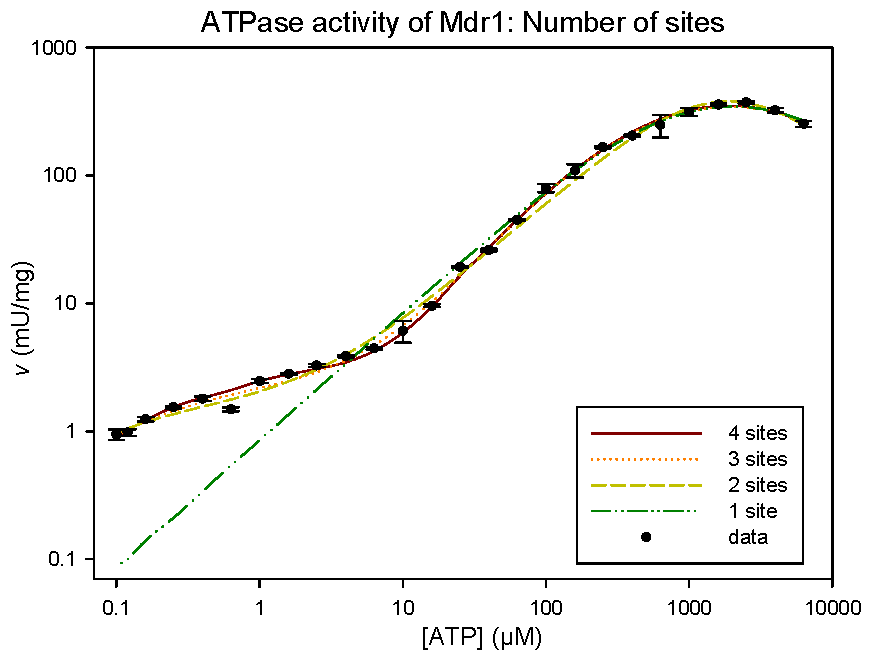
\includegraphics[width=\textwidth]{Graphics/ATPase-sites}
\end{figure}

To determine the number of ATP-binding sites in Mdr1 the substrat/velocity curve was measured (see fig. \ref{fig:ATPsites}). As shown already in  fig. \ref{fig:ATPase}, these data cannot be fitted by the least squares criterium, but the \(\chi^2\)-criterium works very well. Relative errors were used throughout the analysis. Increasing the number of sites (and hence the order of the ratio of polynoms) results in more flexible curves, and hence a better fit to the data. However, this may be caused by a fit to the noise (overfitting). Results for models with 1--4 catalytic binding sites, plus a site for substrate inhibition are summarised in this table, \( \nu_1 = 24,\quad \nu_2 = 212,\quad q_2 = 2079.4 \):

\begin{tabular}{rrrrr}
  \toprule
               & 1 site         & 2 sites             & 3 sites        & 4 sites      \\
  \midrule

  \skalar{q_1} & \num{54762.6}  & \num{3894.0}        & \num{2290.1}   & \num{603.2}  \\
  F            & \num{232.6}    & \num{16.5}          & \num{9.73}     & \num{1.56}   \\
  P(0) \%      & \(<0.1\)       & \(<0.1\)            & \(<0.1\)       & \num{5.2}    \\
 \bottomrule
\end{tabular}

The \(F\)-test shows that curves for 1--3 catalytic binding sites do not explain the data well, we can reject \skalar{H_0} (the residuals can be explained by the standard deviation of the data) with an error probability of less than \SI{0.1}{\%}. For a model with 4 catalytic sites, on the other hand, the null-hypothesis is accepted at the \SI{5}{\%} level. Thus, Mdr1 must have at least four kinetically different binding sites for ATP. We cannot be sure wether it is only four sites or even more; but we can exclude models with fewer sites.

For the runs test the one-site model gives us \(+-----++-+-++++++----------\), the two-site model  \(---+++-------++++---+--+-\), the three-site model  \(+---+++-+--+-+++----+---+-\) and four-site model \(+---+++-+-++--------+++++-\). Thus, we get

\begin{tabular}{rrrrr}
  \toprule
                &  1    &  2    &  3    &   4    \\
  \midrule
  \(n_+\)       & 10    &  9    & 11    &  12    \\
  \(n_-\)       & 16    & 17    & 15    &  14    \\
  \(n\)         & 26    & 26    & 26    &  26    \\
  \(R_o\)       &  9    &  9    & 14    &  10    \\
  \(R_e\)       & 13.3  & 12.8  & 13.7  &  11.9  \\
  \(\sigma_R\)  &  1.42 &  5.07 &  5.94 &   6.16 \\
  \(Z\)         &  2.68 &  0.64 &  0.16 &   0.23 \\
  \bottomrule
  \(P_0\) \si{\%}& 0.37 & 25.1  & 43.6  &  40.9  \\
  \bottomrule
\end{tabular}

In other words, we can reject the one-site model (even if not at the same high confidence as with the \(F\)-test), but we cannot see a significant improvement beyond the 2-site model. This lower sensitivity of the runs test is typical for non-parametric compared to parametric tests. On the other hand, non-parametric tests are a lot less work!

\section{Code for Simplex-Regression}

The following program was modified from \parencite{Nel-65,Cac-84}. The formula compiler was published in \parencite{Gie-87b}, error limit determination by Monte-Carlo simulation was described in \parencite{Str-92}.

\begin{lstlisting}[caption=Simplex]
  UNIT SimplexFit;

  {Regressionsanalyse nach M.Caceci, W.P. Cacheris: Fitting Curves to Data,
        Byte Magazine May 1984, S. 340-350
   Unter Benutzung des Formel-Compilers aus Pascal International 8/1987, S. 52-60
   Die Bestimmung der Fehlergrenzen durch Monte-Carlo-Simulation ist beschrieben
        von Straume & Johnson, Meth. Enzymol. 210 (1992) 117-129
   Die Idee der Minimierung von Chi2 für Daten mit bekannten Fehlergrenzen stammt
        aus Press et al.: Numerical Recepies in Pascal, Cambridge 1989
   Gesamtprogramm copyright 1988-1994 by Dr. Engelbert Buxbaum }

  INTERFACE

  USES MathFunc,            // basic maths
       crt,                 // low level system calls
       Calc,                // formula compiler
       Vector,              // vector arithmetic
       Matrix,              // matrix arithmetic
       Deskript,            // descriptive statistics
       Zufall               // random numbers
       ;

  CONST
    SimplexError: BOOLEAN = FALSE;

  PROCEDURE Approximation(Data: MatrixTyp; VAR yBerech: VectorTyp;
    VAR ProblemName, Formel, xName, yName: STRING);


  IMPLEMENTATION

  CONST
    alfa                  = 1.0;                 // Reflektion coefficient
    beta                  = 0.5;                 // Kontraktion coefficient
    gamma                 = 2.0;                 // Expansion coefficient
    MaxParameter          = 10;
    MaxVariablen          = 10;
    MaxN                  = MaxParameter + 1;    // dimension of simplex
    lw                    = 5;                   // linewidth of data field + 1
    Page                  = 12;
    Ja                    = 'Y';                 // key for yes
    Nein                  = 'N';                 // key for no

  var ch : char;                                     // for error handling

  PROCEDURE Approximation(Data: MatrixTyp; VAR yBerech: VectorTyp;
    VAR ProblemName, Formel, xName, yName: STRING);

  TYPE
    AVektor = ARRAY[1..MaxN] OF float;
    DataRow = ARRAY [1..MaxVariablen] OF float;
    simpl   = ARRAY [1..MaxN] OF AVektor;            // Simplex
    ParFeld = ARRAY [1..MaxParameter] OF STRING[10];
    VarFeld = ARRAY [1..MaxVariablen] OF STRING[10];

  VAR
    FehlerGrenzen,                    // Letzte Spalte der Daten-Matrix Fehlergrenzen?
    done: BOOLEAN;                    // Konvergenz

    i, j, n: BYTE;

    h, l: ARRAY [1..MaxN] OF BYTE;    // Zahl Hoch/Niedrig Parameter

    Daten,                            // Zahl der Datenpunkte
    MaxIter,                          // max.Zahl der Iterationen
    NIter: WORD;                      // Zahl der Iterationen

    Next,                             // neuer Vertex zu testen
    center,                           // Minimum aller Vertexe}
    mean, error, MaxErr,              // Maximal zulaessiger Fehler}
    p, q,                             // um ersten Simplex zu berechnen
    step: AVektor;                    // Eingabe Startschritte

    simp: simpl;                      // Simplex

    NameA,                            // Name des Eingabefiles
    NameB: STRING[64];                // Name des Ausgabefiles

    Eindat,                           // Eingabefile
    Ausdat: TEXT;                     // Ausgabefile}

    x: Calc_VarTab;                   // FOR formula compiler
    dummy, Sigma: float;              // y-Standardabweichung
    Formula: Calc_String;
    FormProg: Calc_Prog;

    Variablen, Parameter: BYTE;

    ErrorStat,                        // TRUE wenn Fehlerstatistik gewuenscht
    Erster: BOOLEAN;                  // Startsimplex nur einmal ausgeben

    Antwort: CHAR;

    Methode: (Summe, Median, ChiSqr);  // was soll minimiert werden?


    {****************************************************************************}

    PROCEDURE LiesFunction(VAR x: Calc_VarTab; VAR Formula: Calc_String;
    VAR FormProg: Calc_Prog);

    VAR
      i: BYTE;
      dummy: float;
      Name: Calc_IdStr;
      Input : TEXT;


      PROCEDURE Hilfe;

      BEGIN
        Writeln('The function used for fitting to the data should be entered in the ');
        Writeln('following manner: ');
        Writeln('1) Number and names of the variables (i. e. measured data)');
        Writeln('2) Number and name(s) of the parameters');
        Writeln('3) The formula itself. All names must be entered exactly as defined.');
        Writeln('   No undefined names are allowed. The formula must end with a ');
        Writeln('   semicolon.');
        Writeln;
        Writeln('The compiler ''knows'' the following constants and and functions, which ');
        Writeln('can not be redefined:');
        Writeln('Constants: e, pi                        Basic operators: +, -, *, /, ^');
        Writeln('Integer: div, mod, ggt, kgv             Logarithms: ln, lg, ld, exp');
        Writeln('sin, cos, tan, cot and the equivalent hyperbolic and arcus functions');
        Writeln('Various Functions: abs, deg, rad, fak, sgn');
        Writeln;
      END;


    BEGIN
      Hilfe;
      Assign(Input, 'CON');
      Reset(Input);
      IF SimplexError THEN EXIT;
      CalcDecMod := TRUE;                     {nur definierte Vars und Parms}
      x := NewVarTab;
      Writeln('Data file has ', MatrixColumns(Data), 'columns');
      IF MatrixColumns(Data) > 2
        THEN
          BEGIN
            Write('Last column independend variable or error margin (v/e):');
            REPEAT
              Readln(Antwort);
              Antwort := UpCase(Antwort);
            UNTIL (Antwort IN ['V', 'F', 'E', #27]);
            IF Antwort = #27
              THEN
                BEGIN
                  SimplexError := TRUE;
                  EXIT;
                END;
            FehlerGrenzen := (Antwort = 'F') OR (Antwort = 'E');
          END
        ELSE
          FehlerGrenzen := FALSE;
      IF FehlerGrenzen
        THEN Variablen := Pred(MatrixColumns(Data))
        ELSE Variablen := MatrixColumns(Data);
      Daten := MatrixRows(Data);
      FOR i := 1 TO Pred(Variablen) DO
        BEGIN
          Write('Name of the ', i, '. (independent) variable: ');
          Readln(Name);
          dummy := AddToVarTab(x, Name);
        END;
      Write('Name of the ', Variablen, '. (dependent) variable: ');
      Readln(Name);
      dummy := AddToVarTab(x, Name);
      Write('How many parameters do you want to use [1..', MaxParameter, ']: ');
      ReadLn(Parameter);
      N := Parameter + 1;               {Dimensionen des Simplex}
      FOR i := 1 TO Parameter DO
        BEGIN
          Write('Name of the ', i, '. parameter: ');
          ReadLn(Name);
          dummy := AddToVarTab(x, Name);
        END;
      REPEAT
        Writeln('Please enter the equation: ');
        Writeln;
        Write(x^[Variablen].VarId, ' = ');
        ReadLn(Formula);
        CompileExpression(Formula, x, FormProg);
        IF NOT CalcResult
          THEN Writeln('Unable to compile the equation, please try again: ');
      UNTIL CalcResult;
      Formel := x^[Variablen].VarID + ' = ' + Formula;
      xName := x^[1].VarID;
      yName := x^[Variablen].VarID;
    END;


    FUNCTION f(p: AVektor; d: MatrixTyp; Zeile: WORD): float;

    VAR
      i: BYTE;

    BEGIN
      FOR i := 1 TO Variablen DO
        AssignVar(x, x^[i].VarId, GetMatrixElement(d, Zeile, i));
      FOR i := 1 TO Parameter DO
        AssignVar(x, x^[Variablen + i].VarId, p[i]);
      Result := CalcExpression(FormProg, x);
    END;


    PROCEDURE Inparam(VAR MaxIter: WORD; VAR simp: Simpl; VAR Step, MaxErr: AVektor);
    {Einlesen aller benutzerdefinierten Parameter}

    VAR
      FalscheEingabe: BOOLEAN;
      Quelle: CHAR;
      i: WORD;
      c: CHAR;

    BEGIN
      Writeln('This routine calculates curve fits by the simplex algorithm');
      Writeln;
      LiesFunction(x, Formula, FormProg);
      IF SimplexError THEN EXIT;
      REPEAT
        FalscheEingabe := FALSE;
        Writeln;
        Write('Please enter the name of the output file: ');
        ReadLn(NameB);
        Assign(Ausdat, NameB);
        Rewrite(Ausdat);
        IF IOResult <> 2
          THEN   { d. h., Datei existiest schon }
            BEGIN
              REPEAT
                Write(NameB, ' already exists. Overwrite (y/n): ');
                ReadLn(c);
                c := UpCase(c);
              UNTIL (c = JA) OR (c = Nein) OR (c = #27);
            IF (c = #27)
              THEN
                BEGIN
                  SimplexError := TRUE;
                  EXIT;
                END;
            FalscheEingabe := (c = Nein);
          END;
      UNTIL NOT FalscheEingabe;
      Rewrite(Ausdat);
      Write(Ausdat, 'best fit for equation: ');
      Writeln(Ausdat, x^[Variablen].VarId, ' = ', Formula);
      Writeln(Ausdat);
      REPEAT
        FalscheEingabe := FALSE;
        REPEAT
          IF FehlerGrenzen
            THEN Write('Minimise sum of squares, median of squares or Chi2 (S/M/X): ')
            ELSE Write('Minimise sum or median of squares (S/M): ');
          ReadLn(c);
          c := UpCase(c);
          IF NOT ((c = 'S') OR (c = 'M') OR (c = 'X') OR (c = #27))
            THEN
              BEGIN
                Sound(400);
                Delay(50);
                NoSound;
              END;
        UNTIL (c = 'S') OR (c = 'M') OR (c = 'X') OR (c = #27);
        CASE c OF
          'S': BEGIN
                 Methode := Summe;
                 Writeln(Ausdat, 'Minimising sum of squared residuals ');
               END;
          'M': BEGIN
                 Methode := Median;
                 Writeln(Ausdat, 'Minimising median of squared residuals ');
               END;
          'X': BEGIN
                 IF FehlerGrenzen
                   THEN
                     BEGIN
                       Methode := ChiSqr;
                       Writeln(Ausdat, 'Minimizing Chi2');
                     END
                   ELSE
                     BEGIN
                       ch := WriteErrorMessage('Chi2 erfordert Fehlergrenzen in der letzten Daten-Spalte');
                       SimplexError := TRUE;
                       EXIT;
                     END;
               END;
          #27: BEGIN
                 SimplexError := TRUE;
                 EXIT;
               END;
        END; { case }
        Writeln(Ausdat);
        Write(Ausdat, '                            ');
        FOR i := 1 TO Parameter DO
          Write(Ausdat, x^[i + Variablen].VarId,
            ' ': (ValidFigures + 2 - Length(x^[i + Variablen].VarId)));
        CASE Methode OF
          Summe: Writeln(Ausdat, 'sum of squares ');
          Median: Writeln(Ausdat, 'median of squares');
          ChiSqr: Writeln(Ausdat, 'Chi2');
        END;
      UNTIL NOT FalscheEingabe;
      REPEAT
        FalscheEingabe := FALSE;
        Write('Please enter maximal number of iterations: ');
        ReadLn(MaxIter);
      UNTIL NOT FalscheEingabe;
      REPEAT
        FalscheEingabe := FALSE;
        Writeln('Please enter initial guesses for all parameters: ');
        Write(Ausdat, 'Start coordinates:      ');
        FOR i := 1 TO Parameter DO
          BEGIN
            Write(x^[i + Variablen].VarId, ' = ');
            ReadLn(simp[1, i]);
            IF (i MOD lw) = 0 THEN Writeln(Ausdat);
            Write(Ausdat, FloatStr(simp[1, i], ValidFigures), '  ');
          END;
        Writeln(Ausdat);
        Writeln(Ausdat);
      UNTIL NOT FalscheEingabe;
      REPEAT
        FalscheEingabe := FALSE;
        Writeln('Please enter starting step width for all parameters ');
        Writeln('(ca. 1/10 to 1/2 of initial value)');
        Write(Ausdat, 'Starting step width:    ');
        FOR i := 1 TO Parameter DO
          BEGIN
            Write('Step width:     ', x^[i + Variablen].VarId, ' = ');
            ReadLn(step[i]);
            IF (i MOD lw) = 0 THEN Writeln(Ausdat);
            Write(Ausdat, FloatStr(step[i], ValidFigures), '  ');
          END;
        Writeln(Ausdat);
        Writeln(Ausdat);
        Write(Ausdat, 'max. alowable error:    ');
        FOR i := 1 TO n DO
          BEGIN
            MaxErr[i] := MaxError;
            IF (i MOD lw) = 0 THEN Writeln(Ausdat);
            Write(Ausdat, FloatStr(MaxErr[i], ValidFigures), '  ');
          END;
        Writeln(Ausdat);
        Writeln(Ausdat);
      UNTIL NOT FalscheEingabe;
      REPEAT
        Write('Do you want error margins for the parameters (y/n): ');
        ReadLn(c);
        c := UpCase(c);
      UNTIL (c = JA) OR (c = Nein) OR (c = #27);
      IF (c = #27)
        THEN
          BEGIN
            SimplexError := TRUE;
            EXIT;
          END;
      Writeln(UpCase(c));
      ErrorStat := (c = JA);
    END;


    PROCEDURE sum_of_residuals(VAR z: AVektor; Data: MatrixTyp);
    {Berechnet die Summe der Fehlerquadrate}

    VAR
      i: WORD;

    BEGIN
      z[n] := 0.0;
      FOR i := 1 TO Daten DO
        z[n] := z[n] + Sqr(f(z, Data, i) - GetMatrixElement(Data, i, Variablen));
    END;


    PROCEDURE Median_Of_Squares(VAR z: AVektor; Data: MatrixTyp);
    { berechnet den Median der Fehlerquadrate }

    VAR
      i: WORD;
      Residuals: VectorTyp;

    BEGIN
      CreateVector(Residuals, Daten, 0.0);
      FOR i := 1 TO Daten DO
        SetVectorElement(Residuals, i, Sqr(f(z, Data, i) -
          GetMatrixElement(Data, i, Variablen)));
      ShellSort(Residuals);
      z[n] := Quantile(Residuals, 0.5);
      DestroyVector(Residuals);
    END;

    PROCEDURE Chi(VAR z: AVektor; Data: MatrixTyp);
    {Berechnet chi2}

    VAR
      i: WORD;

    BEGIN
      z[n] := 0.0;
      FOR i := 1 TO Daten DO
        z[n] := z[n] + Sqr(f(z, Data, i) - GetMatrixElement(Data, i, Variablen) /
          GetMatrixElement(Data, i, Succ(Variablen)));
    END;


    PROCEDURE report;
    {berichtet Programstatistik}

     VAR
      dy, h, Zaehler, Nenner, Fehler, Mittel, rSqr: float;
      d1, d2: TEXT;
      HilfsStr: STRING[14];
      i, j: WORD;

    BEGIN
      Writeln(Ausdat);
      Writeln(Ausdat, 'Routine was left after ', NIter: 5, ' iterations');
      Writeln(Ausdat);
      Writeln(Ausdat);
      Writeln(Ausdat, 'The final simplex is: ');
      Write(Ausdat, '                        ');
      FOR j := 1 TO n DO
        BEGIN
          FOR i := 1 TO n DO
            BEGIN
              IF (i MOD lw) = 0 THEN
                Writeln(Ausdat);
              Write(Ausdat, FloatStr(simp[j, i], ValidFigures), '  ');
            END;
          Writeln(Ausdat);
          Write(Ausdat, '                        ');
        END;
      Writeln(Ausdat);
      Write(Ausdat, 'The mean is:            ');
      FOR i := 1 TO n DO
        BEGIN
          IF (i MOD lw) = 0 THEN
            Writeln(Ausdat);
          Write(Ausdat, FloatStr(mean[i], ValidFigures), '  ');
        END;
      Writeln(Ausdat);
      Writeln(Ausdat);
      Write(Ausdat, 'error:                  ');
      FOR i := 1 TO n DO
        BEGIN
          IF (i MOD lw) = 0 THEN
            Writeln(Ausdat);
          Write(Ausdat, FloatStr(error[i], ValidFigures), '  ');
        END;
      Writeln(Ausdat);
      Writeln(Ausdat);
      Write(Ausdat, '  #    ');
      FOR i := 1 TO Variablen DO
        Write(Ausdat, x^[i].VarId, ' ': (ValidFigures + 2 - Length(x^[i].VarId)));
      IF Fehlergrenzen THEN
        Write(Ausdat, 'Delta ', x^[Variablen].VarId, ' ': (ValidFigures -
          2 - Length(x^[i].VarId)));
      Write(Ausdat, x^[Variablen].VarId, ' ber.',
        ' ': (ValidFigures - 2 - Length(x^[Variablen].VarId)));
      Writeln(Ausdat, 'error:                  ');
      Zaehler := 0;
      sigma := 0.0;
      FOR i := 1 TO Daten DO
        BEGIN
          h := f(mean, Data, i);
          SetVectorElement(yBerech, i, h);
          dy := GetMatrixElement(Data, i, Variablen) - h;
          sigma := sigma + Sqr(dy);
          Write(Ausdat, i: 4, '  ');
          FOR j := 1 TO MatrixColumns(Data) DO
            Write(Ausdat, FloatStr(GetMatrixElement(Data, i, j), ValidFigures), '  ');
          Writeln(Ausdat, FloatStr(h, ValidFigures), '  ', FloatStr(dy, ValidFigures));
          Zaehler := Zaehler + GetMatrixElement(Data, i, Variablen);
        END;
      Writeln(Ausdat);
      sigma := Sqrt(sigma / Daten);
      Writeln(Ausdat, 'The standard deviation is:    ', FloatStr(sigma, ValidFigures));
      Fehler := sigma / Sqrt(Daten - Parameter);
      Writeln(Ausdat, 'The error of the function is: ', FloatStr(Fehler, ValidFigures));
      Mittel := Zaehler / Daten;
      Zaehler := 0;
      Nenner := 0;
      FOR i := 1 TO Daten DO
        BEGIN
          Zaehler := Zaehler + Sqr(GetVectorElement(yBerech, i) - Mittel);
          Nenner := Nenner + Sqr(GetMatrixElement(Data, i, Variablen) - Mittel);
        END;
      rSqr := Zaehler / Nenner;
      Writeln(Ausdat, 'r2:                           ', FloatStr(rSqr, ValidFigures));
    END;


    PROCEDURE First;

    VAR
      i, j: WORD;

    BEGIN
      Write(Ausdat, 'Start simplex ');
      FOR j := 1 TO n DO
        BEGIN
          Write(Ausdat, ' simp[', j: 3, ']');
          FOR i := 1 TO n DO
            BEGIN
              IF (i MOD lw) = 0 THEN Writeln(Ausdat);
              Write(Ausdat, FloatStr(simp[j, i], ValidFigures), '  ');
            END;
          Writeln(Ausdat);
          Write(Ausdat, '              ');
        END;
      Writeln(Ausdat);
    END;


    PROCEDURE new_vertex;
    {ersetzt worst durch next}

    VAR
      i, j: WORD;

    BEGIN
      IF erster THEN Write(' --- ', NIter: 4);
      FOR i := 1 TO n DO
        BEGIN
          simp[h[n], i] := Next[i];
          IF erster THEN Write(FloatStr(Next[i], ValidFigures));
        END;
      IF erster THEN Writeln;
    END;


    PROCEDURE order;
    {Highs und Lows fuer jeden Parameter}

    VAR
      i, j: BYTE;

    BEGIN
      FOR j := 1 TO n DO
        BEGIN
          FOR i := 1 TO n DO
            BEGIN
              IF simp[i, j] < simp[l[j], j] THEN l[j] := i;
              IF simp[i, j] > simp[h[j], j] THEN h[j] := i;
            END;
        END;
    END;


    PROCEDURE Iteration(Data: MatrixTyp);

    VAR
      i, j: WORD;

    BEGIN
      NIter := 0;
      REPEAT
        done := TRUE;
        NIter := Succ(NIter);
        FOR i := 1 TO n DO center[i] := 0.0;
        FOR i := 1 TO n DO
          IF i <> h[n]
            THEN
              FOR j := 1 TO Parameter DO
                center[j] := center[j] + simp[i, j];
        FOR i := 1 TO n DO
          BEGIN
            center[i] := center[i] / Parameter;
            Next[i] := (1.0 + alfa) * center[i] - alfa * simp[h[n], i];
          END;
        CASE Methode OF
          Summe: sum_of_residuals(Next, Data);
          Median: Median_Of_Squares(Next, Data);
          ChiSqr: Chi(Next, Data);
        END;
        IF Next[n] <= simp[l[n], n]
          THEN
            BEGIN
              new_vertex;
              FOR i := 1 TO n DO
                Next[i] := gamma * simp[h[n], i] + (1.0 - gamma) * center[i];
              CASE Methode OF
                Summe: sum_of_residuals(Next, Data);
                Median: Median_Of_Squares(Next, Data);
                ChiSqr: Chi(Next, Data);
              END;
              IF Next[n] <= simp[l[n], n] THEN new_vertex;
            END
          ELSE
            BEGIN
              IF Next[n] <= simp[h[n], n]
                THEN
                  new_vertex
                ELSE
                  BEGIN
                    FOR i := 1 TO Parameter DO
                      Next[i] := beta * simp[h[n], i] + (1.0 - beta) * center[i];
                    CASE Methode OF
                      Summe: sum_of_residuals(Next, Data);
                      Median: Median_Of_Squares(Next, Data);
                      ChiSqr: Chi(Next, Data);
                    END;
                    IF Next[n] <= simp[h[n], n]
                      THEN
                        new_vertex
                      ELSE
                        BEGIN
                          FOR j := 1 TO Parameter DO
                            BEGIN
                              simp[i, j] := (simp[i, j] + simp[l[n], j]) * beta;
                              CASE Methode OF
                                Summe: sum_of_residuals(simp[i], Data);
                                Median: Median_Of_Squares(simp[i], Data);
                                ChiSqr: Chi(simp[i], Data);
                              END; // case
                            END; // for j
                        END; // else
                  END; // else
            END; //else
        order;
        FOR j := 1 TO n DO
          BEGIN
            error[j] := (simp[h[j], j] - simp[l[j], j]) / simp[h[j], j];
            IF done
              THEN IF error[j] > MaxErr[j]
                     THEN done := FALSE;
          END;
      UNTIL (done OR (NIter = MaxIter));
    END;


    PROCEDURE DoIteration(VAR Simp: Simpl; Data: MatrixTyp; VAR Mean: AVektor);

    VAR
      i, j: WORD;

    BEGIN
      CASE Methode OF
        Summe: sum_of_residuals(simp[1], Data);
        Median: Median_Of_Squares(simp[1], Data);
        ChiSqr: Chi(simp[1], Data);
      END;
      FOR i := 1 TO Parameter DO
        BEGIN
          p[i] := step[i] * (Sqrt(n) + Parameter - 1) / (Parameter * Sqrt(2));
          q[i] := step[i] * (Sqrt(n) - 1) / (Parameter * Sqrt(2));
        END;
      FOR i := 2 TO n DO
        BEGIN
          FOR j := 1 TO Parameter DO simp[i, j] := simp[1, j] + q[j];
          simp[i, i - 1] := simp[1, i - 1] + p[i - 1];
          CASE Methode OF
            Summe: sum_of_residuals(simp[i], Data);
            Median: Median_Of_Squares(simp[i], Data);
            ChiSqr: Chi(simp[i], Data);
          END;
        END;
      FOR i := 1 TO n DO
        BEGIN
          l[i] := 1;
          h[i] := 1;
        END;
      order;
      IF Erster THEN First;
      Iteration(Data);
      FOR i := 1 TO n DO
        BEGIN
          mean[i] := 0.0;
          FOR j := 1 TO n DO
            mean[i] := mean[i] + simp[j, i];
          mean[i] := mean[i] / n;
        END;
    END;


    PROCEDURE CalculateErrorMargins;

    CONST
      Anzahl = 100;

    VAR
      Counter, Differenz, Ergebniss: AVektor;
      SimulatedData, Ergebnisse: MatrixTyp;
      i, j, k: WORD;


      PROCEDURE Simulate(VAR SimulatedData: MatrixTyp; yBerech: VectorTyp;
        Sigma: float);

      VAR
        i: WORD;
        Wert: float;

      BEGIN
        FOR i := 1 TO MatrixColumns(SimulatedData) DO
          BEGIN
            Wert := RandomLaplace(GetVectorElement(yBerech, i), Sigma);
            SetMatrixElement(SimulatedData, i, Variablen, Wert);
          END;
      END;

    BEGIN
      Sigma := Sqr(Sigma);
      CopyMatrix(Data, SimulatedData);
      CreateMatrix(Ergebnisse, Anzahl, N, 0.0);
      FOR j := 1 TO N DO
        Counter[j] := 0.0;
      FOR i := 1 TO 100 DO
        BEGIN
          Write(i: 3, '  ');
          Simulate(SimulatedData, yBerech, Sigma);
          DoIteration(Simp, SimulatedData, Ergebniss);
          FOR j := 1 TO N DO
            BEGIN
              SetMatrixElement(Ergebnisse, i, j, Ergebniss[j]);
              Counter[j] := Counter[j] + Ergebniss[j];
              Write(FloatStr(Ergebniss[j], ValidFigures), '  ');
            END;
          Writeln;
        END;
      DestroyMatrix(SimulatedData);
      FOR j := 1 TO N DO
        BEGIN
          Counter[j] := Counter[j] / Anzahl;       { Mittelwerte der Parameter }
          Differenz[j] := 0.0;
        END;
      FOR i := 1 TO Anzahl DO
        FOR j := 1 TO N DO
          Differenz[j] := Sqr(Counter[j] - GetMatrixElement(Ergebnisse, i, j));
      Writeln(Ausdat);
      Writeln(Ausdat, 'Standard deviation of the parameters: ');
      Write(Ausdat, '                        ');
      FOR j := 1 TO N DO
        BEGIN
          Differenz[j] := Sqrt(Differenz[j] / Pred(Anzahl));
          IF (j MOD lw) = 0 THEN Writeln(Ausdat);
          Write(Ausdat, FloatStr(Sqrt(Differenz[j]), ValidFigures), '  ');
        END;
      Writeln(Ausdat);
    END;

  BEGIN {Approximation}
    Erster := TRUE;
    Inparam(MaxIter, simp, step, MaxErr);
    IF SimplexError THEN EXIT;
    DoIteration(Simp, Data, Mean);
    CreateVector(yBerech, Daten, 0.0);
    report;
    Erster := FALSE;
    IF ErrorStat THEN CalculateErrorMargins;
    Close(Ausdat);
  END;

  END.
\end{lstlisting}

\begin{lstlisting}[caption=Test program]
  program Simplex;


  USES
    MathFunc,            // basic math functions
    Vector,              // vector arithmetic
    Matrix,              // matrix arithmetic
    Zufall,              // random numbers
    SimplexFit           // curve fit by simplex
    ;

  const MaxData = 100;

  VAR Data                              : MatrixTyp;
      Calculated                        : VectorTyp;
      ProblemName, Formel, xName, yName : STRING;

  { *********************************************************************** }

  PROCEDURE CreateDataSet (VAR Data : MatrixTyp);

  VAR i : WORD;
      x, y : float;

  BEGIN
    FOR i := 1 TO MatrixRows(Data) DO
      BEGIN
        x := i/10 ;
        SetMatrixElement(Data, i, 1, x);
        y := x / (1+x);                  // normalised Henri-Michaelis-Menten law
        y := y + RandomNormal(0, 0.1);   // add normal-distributed random noise
        SetMatrixElement(Data, i, 2, y);
      END;
  END;


  BEGIN {Hauptprogram}
    CreateMatrix(Data, MaxData, 2, 0.0);
    CreateVector(Calculated, MaxData, 0.0);
    CreateDataSet(Data);
    Approximation(Data, Calculated, ProblemName, Formel, xName, yName);
    DestroyMatrix(Data);
    DestroyVector(Calculated);
  END.
\end{lstlisting}


\printbibliography[heading=subbibliography]
\end{refsection}
